\documentclass{article}

\usepackage{biblatex}
\addbibresource{../resources.bib}

\usepackage{graphicx}
\usepackage{tikz}
\usetikzlibrary{arrows}
\usetikzlibrary{quantikz}

\usepackage{physics}
\usepackage{amsthm}

\newtheorem{defn}{Definition}
\newtheorem{thrm}{Theorem}
\newtheorem{prob}{Problem}
\def\F{\mathcal{F}}

\title{Project Progress Report}
\author{Seyed Sajad Kahani \\ 22222815}

\begin{document}
\maketitle

\nocite{*}

\section{Literature Review}

The literature review is divided into three parts: general-purpose quantum compilers, specific-purpose quantum compilers for Hamiltonians, and classical problems and algorithms related to the compilation.

\subsection{General Quantum Compilers}

The first part, consists of papers which are directly related to quantum compilation. While most of the papers are useful for our case, we are also looking for two specific subjects in these papers.

First, we are looking for the approaches to the gate-set specially two-qubit gates through the process of compiling.
Secondly, our aim is to extract the algorithms and principles for qubit allocation, and routing gates through the device.

We have analysed almost all of the papers listed below, in terms of the gate-set, but we are still looking through the papers to organize and categorize their algorithms and their corresponding problems in qubit allocation and routing.

\printbibliography[heading=none,keyword=general]

\subsection{Hamiltonian Quantum Compilers}

Compilation of Hamiltonians has its own literature, although it is not as extensive as that of general quantum compilers. Any paper related to the compilation of Hamiltonians is considered as a part of this section and is being carefully studied.

The paper \cite{lao2021} is being used as a baseline for our project.

\printbibliography[heading=none,keyword=hamiltonian]

\subsection{Classical Compilation and Related Problems}

Many of the problems in designing and implementing quantum compilers have counterparts in the classical world that are well-studied. A deep review of classical compilation is necessary for this project, as well as a search for algorithms from related fields such as resource allocation in distributed systems and scheduling in operating systems.

We have started reviewing the two main books \cite{aho1986} and \cite{allen2001}, and are still looking for additional relevant papers.

\printbibliography[heading=none,keyword=classical]

\section{The Aim}

The objective of this project is to survey the current literature on compiling local Hamiltonians, and use this information to enhance existing approaches, such as 2QAN. In order to effectively tackle the complex compilation process, the sub-problems must be decomposed into smaller and more manageable tasks.

The results of this project will then be tested and evaluated for performance and quality, with the goal of creating a prototype implementation that can be used and further developed by other researchers. It should be noted that the focus will be on exploring solutions rather than creating a polished and highly-engineered implementation.

Note that this objective, is carried on from the beginning of the project, and it is still valid by this time.

\section{Results}

Besides all the insights and the knowledge that we have gained from the literature review, we have also a few ideas that can result in improving the existing compilers.

The main idea which is developed pretty well, is related to the routing problem.

When we have a two-qubit gate, (for example, a CNOT gate), and it shall be applied between two qubits that their corresponding qubits on the device are not connected, we will use a chain of SWAP operators to move the qubits and make them adjacent to each other, and then apply the gate. This is a very common approach \cite{cowtan2019}.

Here we introduce a possible simplification of this approach, using simplified bridge gates, instead of using a chain of SWAP operators.

\subsection{Bridge Gate}

For a simple case, that we have three qubits, called $a, b, c$, and we want to apply a CNOT gate on $(a, c)$, but the connectivity only allows us to apply a CNOT gate on $(a, b)$ and $(b, c)$, the first solution would be to use a SWAP gate, which is shown in figure \ref{fig:bridge-one-with-swap} (7 gates, depth of 7)
While another approach is to use a bridge gate, which is shown in figure \ref{fig:bridge-one-with-bridge} (4 gates, depth of 4). \cite{shende2006}

  \def\qceq{\midstick[3,brackets=none]{=}}
  \begin{figure}[h]
    \label{fig:bridge-one-with-swap}
    \centering
    \begin{quantikz}
    \lstick{a} & \ctrl{2} & \qw \qceq & \swap{1} & \qw & \swap{1} & \qw\qceq & \ctrl{1} & \targ{} & \ctrl{1} & \qw &\ctrl{1} & \targ{} & \ctrl{1} & \qw \\
    \lstick{b} & \qw & \qw & \swap{} & \ctrl{1} & \swap{} & \qw & \targ{} & \ctrl{-1}& \targ{} & \ctrl{1} & \targ{} & \ctrl{-1}& \targ{} & \qw \\
    \lstick{c} & \targ{} & \qw  & \qw & \targ{} & \qw & \qw & \qw & \qw & \qw & \targ & \qw & \qw & \qw & \qw  & \qw \\
    \end{quantikz}
    \caption{Applying a CNOT gate on $(a, c)$ using a SWAP gate}
  \end{figure}

  \begin{figure}[h]
    \label{fig:bridge-one-with-bridge}
    \centering
    \begin{quantikz}
    \lstick{a} & \ctrl{2} & \qw \qceq & \qw & \ctrl{1} & \qw & \ctrl{1} & \qw \\
    \lstick{b} & \qw & \qw & \ctrl{1} & \targ{} & \ctrl{1}  & \targ{} & \qw \\
    \lstick{c} & \targ{} & \qw & \targ{} & \qw  & \targ & \qw  & \qw &  \qw \\
    \end{quantikz}
    \caption{Applying a CNOT gate on $(a, c)$ using a bridge gate}
  \end{figure}
  
  The bridge gate is already generalized using a recursive approach \cite{shende2006}, with $4n + O(1)$ depth and $4n + O(1)$ gates complexity. (where $n$ is the number of qubits in the chain). Here we present a simplified version of the bridge gate, with $n + O(1)$ depth and $4n + O(1)$ gates complexity.

  Note that a simple swapping approach will have $3n + O(1)$ depth and $6n + O(1)$ gates complexity.

  \begin{defn}{Simplified Bridge Gate}
    We can define a simplified bridge gate, recursively, as follows:
    \begin{equation}
      \begin{aligned}
      \mathrm{Bridge}_n(1, n) =& \mathrm{CNOT}(2, 1) \mathrm{CNOT}(1, 2)
      \mathrm{CNOT}(n, n - 1) \mathrm{CNOT}(n - 1, n) \\ &\mathrm{Bridge}_{n - 1}(2, n - 1) \\ &\mathrm{CNOT}(2, 1) \mathrm{CNOT}(1, 2)
      \mathrm{CNOT}(n, n - 1) \mathrm{CNOT}(n - 1, n)
      \end{aligned}
    \end{equation}
    where $\mathrm{Bridge}_2$ is defined as fig. \ref{fig:bridge-one-with-bridge} and $\mathrm{Bridge}_1$ is just a CNOT.
  \end{defn}

  We ignore to show that this gate is equivalent to the recursive definition of the bridge gate, since it is not the main focus of the progress report.

  It is easy to show that such circuit contains $4n + O(1)$ gates, but in order to show the depth, we need to use the fact that two CNOTs applying on the same gates, commute with each other, therefore, like for the case of even $n$s, we can show the recursive formula is equivalent to the following:
    \begin{equation}
      \begin{aligned}
      \mathrm{Bridge}_n(1, n) = &\prod_{i=1}^{n/2 - 1}\mathrm{CNOT}(i + 1, i)\mathrm{CNOT}(n - i + 1, n - i) \\ & \prod_{i=1}^{n/2 - 1}\mathrm{CNOT}(i, i + 1)\mathrm{CNOT}(n - i, n - i + 1) \\ & \mathrm{Bridge}_1(n/2 - 1, n/2)  \\
    & \qty(\prod_{i=1}^{n/2 - 1}\mathrm{CNOT}(i + 1, i)\mathrm{CNOT}(n - i + 1, n - i))^\dagger \\ 
    & \qty(\prod_{i=1}^{n/2 - 1}\mathrm{CNOT}(i, i + 1)\mathrm{CNOT}(n - i, n - i + 1))^\dagger
      \end{aligned}
    \end{equation}

    where each term of each products in the RHS and the LHS can be applied simultaneously (4 gates at a time).
    Therefore, the depth of the circuit is $n + O(1)$.
    Hereby we can see an example of the bridge gate for $n = 6$ in fig. \ref{fig:bridge-simplified}.
  \def\qceq{\midstick[6,brackets=none]{=}}
  \begin{figure}[h]
    \centering
\begin{quantikz}
\qw &\ctrl{5}&\qw\qceq&\targ{}  & \qw     &\ctrl{1}& \qw    & \qw    & \qw    &\ctrl{1}& \qw     &\targ{}&\qw\\
\qw & \qw    & \qw    &\ctrl{-1}&\targ{}  & \targ{}&\ctrl{1}& \qw    &\ctrl{1}&\targ{} &\targ{}  &\ctrl{-1}&\qw\\
\qw & \qw    & \qw    & \qw     &\ctrl{-1}& \qw    & \targ{}&\ctrl{1}&\targ{} & \qw    &\ctrl{-1}&\qw & \qw \\
\qw & \qw    & \qw    & \qw     &\targ{}  & \qw    &\ctrl{1}& \targ{}&\ctrl{1}& \qw    &\targ{}  &\qw & \qw\\
\qw & \qw    & \qw    &\targ{}  &\ctrl{-1}&\ctrl{1}& \targ{}& \qw    &\targ{} &\ctrl{1}&\ctrl{-1}&\targ{}&\qw \\
\qw &\targ{} & \qw    &\ctrl{-1}& \qw     & \targ{}& \qw    & \qw    & \qw    &\targ{} & \qw     &\ctrl{-1}& \qw 
\end{quantikz}
    \caption{The bridge gate for $n=6$}
    \label{fig:bridge-simplified}
  \end{figure}

  Furthermore, we can use the same idea and create a bridge gate to express $e^{iZ^{1}X^{n}}$ using CNOTs and $e^{iZ^{1}X^{2}}$ gates. Then we are working on the most general way to bridge a qubit gate between two qubits in a chain.

  It is also proved that any effort to decompose a CNOT into a chain of CNOTs, cannot result in any complexity better than the simplified bridge gate. Therefore, the simplified bridge gate is the best possible gate to bridge a qubit gate between two qubits in a chain.

  As far as we know, the family of bridge gates (the previous one or the simplified one) is not implemented (explicitly or implicitly) in any quantum compiler. 
  It can be easily shown that for a simple case like the one in the figure \ref{fig:bridge-simplification} that we need to swap and return the qubits, using bridge gate can reduce both depth and number of gates.

  \begin{figure}
    a) \\
    \begin{center}
    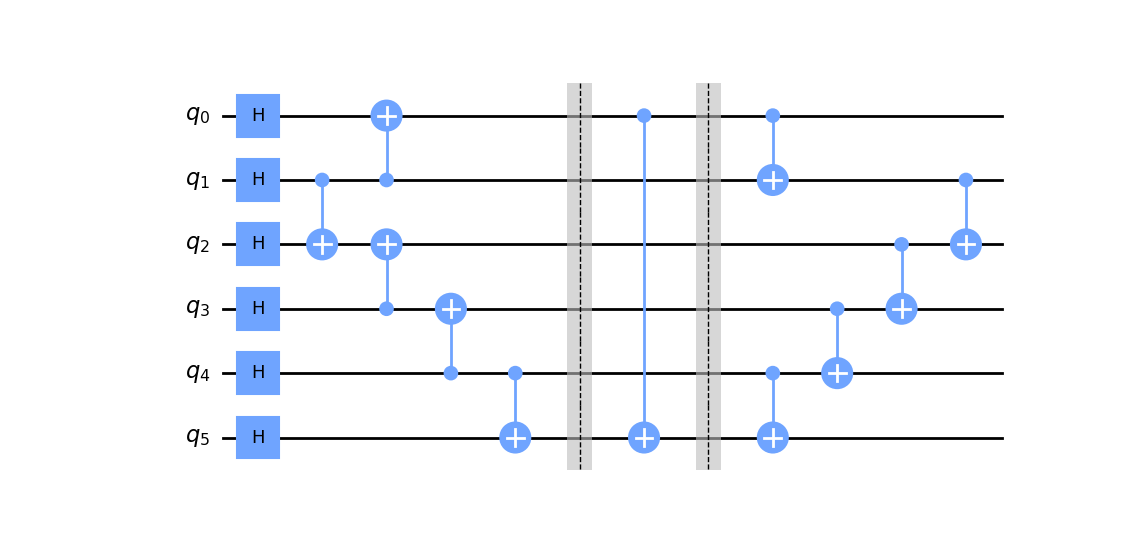
\includegraphics[width=0.9\textwidth]{../../code/expm_1_bridge/out/original_circuit}
    \end{center}
    b) \\
    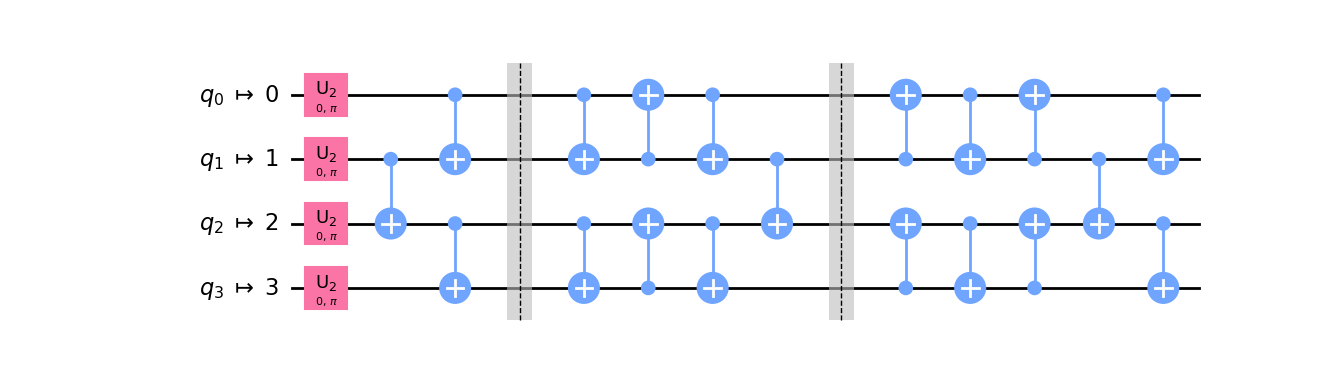
\includegraphics[width=0.9\textwidth]{../../code/expm_1_bridge/out/transpiled_circuit_swap} \\
    c) \\
    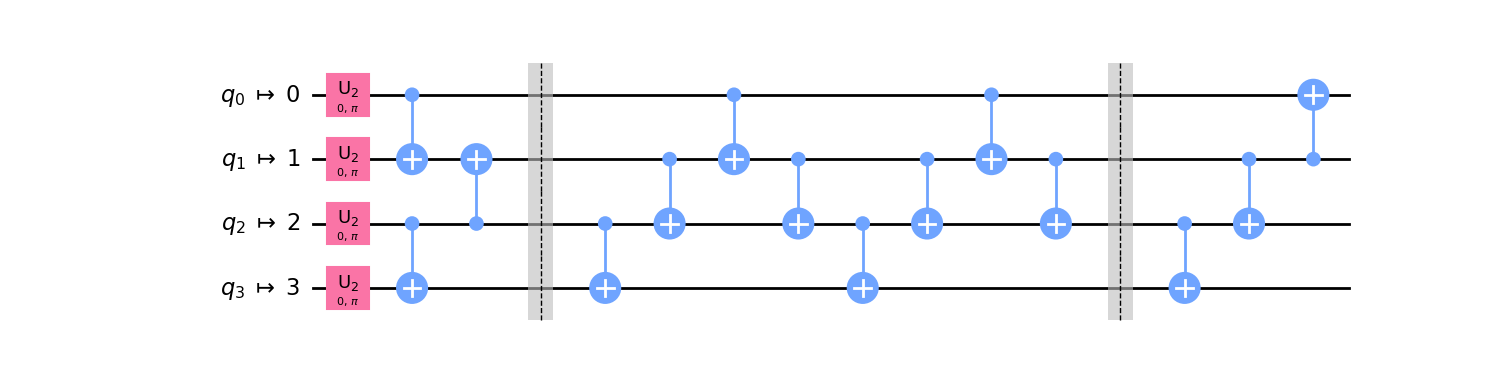
\includegraphics[width=0.9\textwidth]{../../code/expm_1_bridge/out/transpiled_circuit_bridge}
    \caption{a) The original circuit, consisting of some local operations, then a far away CNOT and then some local operations. b) The circuit after transpiling using Qiskit. c) The circuit after transpiling using bridge gate as an intermediate gate.}
  \end{figure}

\section{Challenges}

\begin{itemize}
\item Interdisciplinary work, a wide range of keywords, a wide range of languages in the papers.

\item The subtle line between theoretical works and applicability
\end{itemize}


\end{document}